Artificial intelligence is a pretty useful tool, as long as it doesn't
get too smart. Of course, that's the situation you find yourself in now,
as your Piloting ALgorithm (PAL) is afraid
it can't let you direct your ship 
into a particularly dangerous system.

PAL concedes that it will let you proceed, but only if can solve 
the puzzle of its \textbf{Cubic Monolith}.
To do so, you'll need to adhere to the illustrated rules for
placing the numbers \(1\) through \(3\) in the grids.
%
%\begin{itemize}
%\item Rule 1: Each row of a level must contain exactly one
%  of the numbers 1,2,3,4.
%\item Rule 2: Each column of a level must contain exactly one
%  of the numbers 1,2,3,4.
%\item Rule 3: Each tower of the cube must contain exactly one
%  of the numbers 1,2,3,4.
%\item Rule 4: All the numbers within each solid-boundary cage
%  (possibly connected by arrows to other levels) of the cube 
%  either add or multiply to 12.
%\end{itemize}

\begin{center}
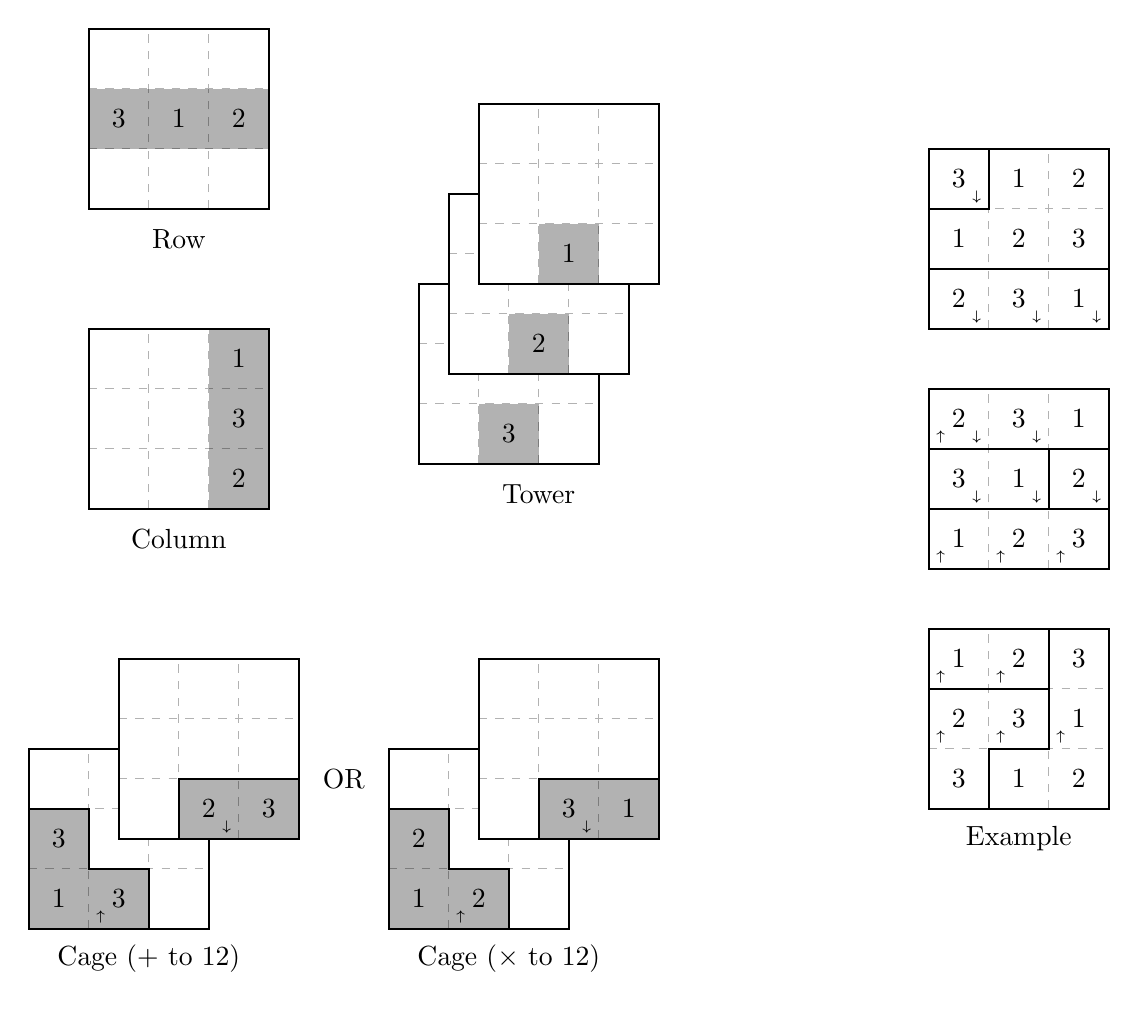
\begin{tikzpicture}[x=0.3in,y=0.3in]
\begin{scope}[shift={(-1,0)}]
\draw[fill=white] (0,0) rectangle (3,3);
\draw[step=1,dashed,color=black!30] (0,0) grid (3,3);
\draw[thick] (0,0) rectangle (3,3);
\fill[opacity=0.3] (0,1) rectangle (3,2);
\node at (1.5,-0.5) {Row};
\node at (0.5,1.5) {3};
\node at (1.5,1.5) {1};
\node at (2.5,1.5) {2};
\end{scope}
\begin{scope}[shift={(-1,-5)}]
\draw[fill=white] (0,0) rectangle (3,3);
\draw[step=1,dashed,color=black!30] (0,0) grid (3,3);
\draw[thick] (0,0) rectangle (3,3);
\fill[opacity=0.3] (2,0) rectangle (3,3);
\node at (1.5,-0.5) {Column};
\node at (2.5,0.5) {2};
\node at (2.5,1.5) {3};
\node at (2.5,2.5) {1};
\end{scope}
\begin{scope}[shift={(4.5,-4.25)}]
\draw[fill=white] (0,0) rectangle (3,3);
\draw[step=1,dashed,color=black!30] (0,0) grid (3,3);
\draw[thick] (0,0) rectangle (3,3);
\fill[opacity=0.3] (1,0) rectangle (2,1);
\node at (2,-0.5) {Tower};
\node at (1.5,0.5) {3};
%\node[right,black!30] at (3,0.5) {Bottom Level};
  \begin{scope}[shift={(0.5,1.5)}]
  \draw[fill=white] (0,0) rectangle (3,3);
  \draw[step=1,dashed,color=black!30] (0,0) grid (3,3);
  \draw[thick] (0,0) rectangle (3,3);
  \fill[opacity=0.3] (1,0) rectangle (2,1);
  \node at (1.5,0.5) {2};
  \begin{scope}[shift={(0.5,1.5)}]
  \draw[fill=white] (0,0) rectangle (3,3);
  \draw[step=1,dashed,color=black!30] (0,0) grid (3,3);
  \draw[thick] (0,0) rectangle (3,3);
  \fill[opacity=0.3] (1,0) rectangle (2,1);
  \node at (1.5,0.5) {1};
  \end{scope}
  \end{scope}
\end{scope}
\begin{scope}[shift={(-2,-12)}]
\draw[fill=white] (0,0) rectangle (3,3);
\draw[step=1,dashed,color=black!30] (0,0) grid (3,3);
\draw[thick] (0,0) rectangle (3,3);
\fill[opacity=0.3] (0,2) -- (1,2) -- (1,1) -- (2,1) -- (2,0) -- (0,0) -- (0,2);
\draw[thick] (0,2) -- (1,2) -- (1,1) -- (2,1) -- (2,0);
\node at (2,-0.5) {Cage (\(+\) to \(12\))};
\node at (1.5,0.5) {3};
\node at (0.5,0.5) {1};
\node at (0.5,1.5) {3};
\node at (1.2,0.2) {\tiny\(\uparrow\)};
  \begin{scope}[shift={(1.5,1.5)}]
  \draw[fill=white] (0,0) rectangle (3,3);
  \draw[step=1,dashed,color=black!30] (0,0) grid (3,3);
  \draw[thick] (0,0) rectangle (3,3);
  \draw[thick] (1,0) rectangle (3,1);
  \fill[opacity=0.3] (1,0) rectangle (3,1);
  \node at (1.5,0.5) {2};
  \node at (2.5,0.5) {3};
  \node at (1.8,0.2) {\tiny\(\downarrow\)};
  \end{scope}
\end{scope}
\node at (3.25,-9.5) {OR};
\begin{scope}[shift={(4,-12)}]
\draw[fill=white] (0,0) rectangle (3,3);
\draw[step=1,dashed,color=black!30] (0,0) grid (3,3);
\draw[thick] (0,0) rectangle (3,3);
\fill[opacity=0.3] (0,2) -- (1,2) -- (1,1) -- (2,1) -- (2,0) -- (0,0) -- (0,2);
\draw[thick] (0,2) -- (1,2) -- (1,1) -- (2,1) -- (2,0);
\node at (2,-0.5) {Cage (\(\times\) to \(12\))};
\node at (1.5,0.5) {2};
\node at (0.5,0.5) {1};
\node at (0.5,1.5) {2};
\node at (1.2,0.2) {\tiny\(\uparrow\)};
  \begin{scope}[shift={(1.5,1.5)}]
  \draw[fill=white] (0,0) rectangle (3,3);
  \draw[step=1,dashed,color=black!30] (0,0) grid (3,3);
  \draw[thick] (0,0) rectangle (3,3);
  \draw[thick] (1,0) rectangle (3,1);
  \fill[opacity=0.3] (1,0) rectangle (3,1);
  \node at (1.5,0.5) {3};
  \node at (2.5,0.5) {1};
  \node at (1.8,0.2) {\tiny\(\downarrow\)};
  \end{scope}
\end{scope}
\begin{scope}[shift={(13,-10)}]
\draw[fill=white] (0,0) rectangle (3,3);
\draw[step=1,dashed,color=black!30] (0,0) grid (3,3);
\draw[thick] (0,0) rectangle (3,3);
\draw[thick] (1,0) -- (1,1) -- (2,1) -- (2,3);
\draw[thick] (0,2) -- (2,2);
\node at (0.2,2.2) {\tiny\(\uparrow\)};
\node at (0.2,1.2) {\tiny\(\uparrow\)};
\node at (1.2,1.2) {\tiny\(\uparrow\)};
\node at (1.2,2.2) {\tiny\(\uparrow\)};
\node at (2.2,1.2) {\tiny\(\uparrow\)};
\node at (1.5,-0.5) {Example};
\node at (0.5,0.5) {3};
\node at (1.5,0.5) {1};
\node at (2.5,0.5) {2};
\node at (0.5,1.5) {2};
\node at (1.5,1.5) {3};
\node at (2.5,1.5) {1};
\node at (0.5,2.5) {1};
\node at (1.5,2.5) {2};
\node at (2.5,2.5) {3};
%\node[right,black!30] at (3,0.5) {Bottom Level};
  \begin{scope}[shift={(0,4)}]
  \draw[fill=white] (0,0) rectangle (3,3);
  \draw[step=1,dashed,color=black!30] (0,0) grid (3,3);
  \draw[thick] (0,0) rectangle (3,3);
  \draw[thick] (0,1) -- (3,1);
  \draw[thick] (0,2) -- (3,2);
  \draw[thick] (2,1) -- (2,2);
  \node at (0.2,0.2) {\tiny\(\uparrow\)};
  \node at (1.2,0.2) {\tiny\(\uparrow\)};
  \node at (2.2,0.2) {\tiny\(\uparrow\)};
  \node at (0.2,2.2) {\tiny\(\uparrow\)};
  \node at (0.8,1.2) {\tiny\(\downarrow\)};
  \node at (1.8,1.2) {\tiny\(\downarrow\)};
  \node at (2.8,1.2) {\tiny\(\downarrow\)};
  \node at (0.8,2.2) {\tiny\(\downarrow\)};
  \node at (1.8,2.2) {\tiny\(\downarrow\)};
  \node at (0.5,0.5) {1};
  \node at (1.5,0.5) {2};
  \node at (2.5,0.5) {3};
  \node at (0.5,1.5) {3};
  \node at (1.5,1.5) {1};
  \node at (2.5,1.5) {2};
  \node at (0.5,2.5) {2};
  \node at (1.5,2.5) {3};
  \node at (2.5,2.5) {1};
  \end{scope}
  \begin{scope}[shift={(0,8)}]
  \draw[fill=white] (0,0) rectangle (3,3);
  \draw[step=1,dashed,color=black!30] (0,0) grid (3,3);
  \draw[thick] (0,0) rectangle (3,3);
  \draw[thick] (0,1) -- (3,1);
  \draw[thick] (0,2) -- (1,2) -- (1,3);
  \node at (0.8,0.2) {\tiny\(\downarrow\)};
  \node at (1.8,0.2) {\tiny\(\downarrow\)};
  \node at (2.8,0.2) {\tiny\(\downarrow\)};
  \node at (0.8,2.2) {\tiny\(\downarrow\)};
  \node at (0.5,0.5) {2};
  \node at (1.5,0.5) {3};
  \node at (2.5,0.5) {1};
  \node at (0.5,1.5) {1};
  \node at (1.5,1.5) {2};
  \node at (2.5,1.5) {3};
  \node at (0.5,2.5) {3};
  \node at (1.5,2.5) {1};
  \node at (2.5,2.5) {2};
  %\node[right,black!30] at (3,0.5) {Top Level};
  \end{scope}
\end{scope}
\end{tikzpicture}
\end{center}
